\documentclass[../mathNotesPreamble]{subfiles}

\providecommand{\relscalefact}{1.4}
\begin{document}
\relscale{\relscalefact}
  \section{1.3: The Language of Relations and Functions}

  \begin{defn*}
    Let $A$ and $B$ be sets. A \textbf{relation $R$ from $A$ to $B$} is a subset of $A\times B$. Given an ordered pair $(x,y)$, \textbf{$x$ is related to $y$ by $R$}, written $\rel{x}{y}$, if, and only if, $(x,y)$ is in $R$. The set $A$ is called the \textbf{domain} of $R$ and the set $B$ is called its \textbf{co-domain}.

    The notation for a relation $R$ may be written symbolically as follows:
      \[\rel{x}{y} \textnormal{ means that } (x,y)\in R.\]
    The notation $\notrel{x}{y}$ means that $x$ is not related to $y$ by $R$:
      \[\notrel{x}{y} \textnormal{ means that } (x,y)\not\in R.\]
  \end{defn*}
  \begin{ex*}
    Let $A=\set{1,2}$ and $B=\set{1,2,3}$ and define a relation $R$ from $A$ to $B$ as follows; Given any $(x,y)\in A\times B$,
      \[(x,y)\in R \textnormal{ means that } \dfrac{x-y}{2} \textnormal{ is an integer.}\]
  \end{ex*}
  \begin{extasks}[after-item-skip=\stretch{1}](3)
    \task* State explicitly which ordered pairs are in $A\times B$ and which are in $R$
    \task Is $\rel{1}{3}$?
    \task Is $\rel{2}{3}$?
    \task Is $\rel{2}{2}$?
    \task* What are the domain and co-domain of $R$?
  \end{extasks}
  \vspace*{\stretch{1}}
  \pagebreak

  \begin{ex*}
    Define a relation $C$ from $\bbr$ to $\bbr$ as follows: For any $(x,y)\in\bbr\times\bbr$,
      \[(x,y)\in C \textnormal{ means that } x^2+y^2=1.\]
  \end{ex*}
  \begin{extasks}[after-item-skip=\stretch{1}](3)
    \task Is $(1,0)\in C$?
    \task Is $(0,0)\in C$?
    \task Is $\parens{-\frac{1}{2},\frac{\sqrt{3}}{2}}\in C$?
    \task Is $\rel[C]{-2}{0}?$
    \task Is $\rel[C]{0}{(-1)}?$
    \task Is $\rel[C]{1}{1}?$
    \task* What are the domain and co-domain of $C$?
    \task* Draw a graph for $C$ by plotting the points of $C$ in the Cartesian plane.
  \end{extasks}
  \vspace*{\stretch{1}}
  \pagebreak

  \begin{defn*}
    Suppose $R$ is a relation from set $A$ to a set $B$. The \textbf{arrow diagram for $R$} is obtained as follows:
    \begin{enumerate}
      \item Represent the elements of $A$ as points in one region and the elements of $B$ as points in another region.
      \item For each $x$ in $A$ and $y$ in $B$, draw an arrow from $x$ to $y$ if, and only if, $x$ is related to $y$ by $R$.
    \end{enumerate}
    \vspace*{-1.2\baselineskip}
    \begin{center}
      \begin{tikzpicture}[
        myPoint/.style={circle, fill, inner sep=1pt},
        myArrow/.style={->, shorten >=7.5pt, shorten <=5pt}]
        \draw (-2,0) circle [x radius=1, y radius=2];
        \draw (2,0) circle [x radius=1, y radius=1.75];
        \node[myPoint, label=$x_1$] (xo) at (-2,1) {};
        \node[myPoint, label=$x_2$] (xt) at (-2,-0.2) {};
        \node[myPoint, label=$x_3$] (xr) at (-2,-1.4) {};
        \node[myPoint, label=$y_1$] (fxo) at (2,0.75) {};
        \node[myPoint, label=$y_2$] (fxt) at (2,-0.85) {};
%        \draw[myArrow] (xo) to (fxo);
        \draw[myArrow] (xt) to (fxo);
        \draw[myArrow] (xt) to (fxt);
        \draw[myArrow] (xr) to (fxt);
        \node (R) at (0,2.2) {$\rel{x}{y}$};
        \draw[->] ($(R)+(-0.75,-0.55)$) to [bend left] ($(R)+(0.75,-0.55)$);
      \end{tikzpicture}
    \end{center}
  \end{defn*}

  \begin{ex*}
    Let $A=\set{1,2,3}$ and $B=\set{1,3,5}$ and define relations $S$ and $T$ from $A$ to $B$ as follows: For every $(x,y)\in A\times B$,
    \begin{align*}
      &(x,y)\in S \textnormal{ means that } x<y\\
      &T=\set{(2,1),(2,5)}.
    \end{align*}
    Draw arrow diagrams for $S$ and $T$
  \end{ex*}
  \vspace*{\stretch{1}}

  \hspace*{\stretch{0.5}}
  \begin{tikzpicture}[
    myPoint/.style={circle, fill, inner sep=1pt}]
    \draw (-2,0) circle [x radius=1, y radius=2];
    \draw (2,0) circle [x radius=1, y radius=2];
    \node[myPoint, label={180:$1$}] (xo) at (-1.8,1) {};
    \node[myPoint, label={180:$2$}] (xt) at (-1.8,0) {};
    \node[myPoint, label={180:$3$}] (xr) at (-1.8,-1) {};
    \node[myPoint, label={0:$1$}] (fxo) at (1.8,1) {};
    \node[myPoint, label={0:$3$}] (fxt) at (1.8,0) {};
    \node[myPoint, label={0:$5$}] (fxt) at (1.8,-1) {};
    \node (S) at (0,2.2) {$S$};
    \draw[->] ($(S)+(-0.75,-0.55)$) to [bend left] ($(S)+(0.75,-0.55)$);
  \end{tikzpicture}
  \hspace*{\stretch{1}}
  \begin{tikzpicture}[
    myPoint/.style={circle, fill, inner sep=1pt}]
    \draw (-2,0) circle [x radius=1, y radius=2];
    \draw (2,0) circle [x radius=1, y radius=2];
    \node[myPoint, label={180:$1$}] (xo) at (-1.8,1) {};
    \node[myPoint, label={180:$2$}] (xt) at (-1.8,0) {};
    \node[myPoint, label={180:$3$}] (xr) at (-1.8,-1) {};
    \node[myPoint, label={0:$1$}] (fxo) at (1.8,1) {};
    \node[myPoint, label={0:$3$}] (fxt) at (1.8,0) {};
    \node[myPoint, label={0:$5$}] (fxt) at (1.8,-1) {};
    \node (T) at (0,2.2) {$T$};
    \draw[->] ($(T)+(-0.75,-0.55)$) to [bend left] ($(T)+(0.75,-0.55)$);
  \end{tikzpicture}
  \hspace*{\stretch{0.5}}
  \pagebreak

  \begin{defn*}
    A \textbf{function $F$ from a set $A$ to a set $B$} is a relation with domain $A$ and co-domain $B$ that satisfies the following two properties:
    \begin{enumerate}
      \item For every element $x$ in $A$, there is an element $y$ in $B$ such that $(x,y)\in F$.
      \item For all elements $x$ in $A$ and $y$ and $z$ in $B$,
        \[\textnormal{ if } (x,y) \in F \textnormal{ and } (x,z) \in F, \textnormal{ then } y=z.\]
    \end{enumerate}
  \end{defn*}

  \emph{Note}: A relation from $A$ to $B$ is a function if, and only if,
  \begin{enumerate}
    \item Every element of $A$ is the first element of an ordered pair of $F$
    \item No two distinct ordered pairs in $F$ have the same first element.
  \end{enumerate}

%  \emph{Note}: We can think of a function as a machine that takes an input and returns a unique output.
  \emph{Note}: If $A$ and $B$ are sets and $F$ is a function from $A$ to $B$, then given any element $x$ in $A$, the unique element in $B$ that is related to $x$ by $F$ is denoted $F(x)$, which is read ``\textbf{$F$ of $x$}''.
  \vspace*{\stretch{1}}

  \noindent
  \begin{minipage}{0.495\linewidth}
    \newcommand{\funcMachine}{--++(0,-vert) --++(dx,-dy) |- ++(-a,-vert) |- ++(c,-h)
      -- ++(0,-vert) --++(-dx, -dy) {[sharp corners] --++(0,-vert-vgap) %bottom left portion
      --++(b+2*dx,0)} --++(0,vert+vgap) --++(-dx,dy) |- ++(a,vert)
      -- ++(0,h) -| ++(-c,vert) --++(dx,dy) --++(0,vert); %top right portion
    }
    \centering
    %bottom left corner is (0,0)
    %a,b,c are widths representing left wall to chute, width of chute, chute to right wall
    %h is height of rectangle
    %dx, dy control slope of "funnel"
    %vert is the height of straight parts of "funnel"
    %paths start at top left (on "funnel")
    \begin{tikzpicture}[declare function={
      a=1.25; b=1.25; c=5.5;
      dx=0.9*a; dy=0.6*a;
      h=1.75; vert=0.6; vgap=0.2;}]
      \begin{scope}
        \clip (-0.1+0,h+2*vert+dy) rectangle ++(0.2+a+b+c,-4*vert-2*dy-h);
        \draw[line width=1pt, fill=lander_blue!25, rounded corners=6pt]
          (a-dx,h+2*vert+dy) \funcMachine
      \end{scope}
      \node (Input) [align=center] at ({a+b/2},{h+vert+dy}) {Input\\$x$};
      \node[align=center] at ({(a+b+c)/2},{h/2}) {$F$};
      \node (Output) [align=center] at ({c+b/2},{-vert-dy}) {$F(x)$\\Output};

      \draw[->] (Input) -- ++(0,-vert-dy);
      \draw[<-] (Output) -- ++(0,vert+dy);
    \end{tikzpicture}
  \end{minipage}\hfill%
  \begin{minipage}{0.495\linewidth}
    \begin{center}
      \begin{tikzpicture}[
        myPoint/.style={circle, fill, inner sep=1pt},
        myArrow/.style={->, shorten >=7.5pt, shorten <=5pt}]
        \draw (-2,0) circle [x radius=1, y radius=2];
        \node at (-2,2.5) {$A$};
        \draw (2,0) circle [x radius=1, y radius=1.75];
        \node at (2,2.25) {$B$};
        \node[myPoint] (xo) at (-2,1) {};
        \node[myPoint] (fxo) at (2,0.5) {};
        \node[myPoint] (xt) at (-2,0) {};
        \node[myPoint] (xr) at (-2,-1) {};
        \node[myPoint] (fxt) at (2,-0.5) {};
        \draw[myArrow] (xo) to [bend left=10] (fxo);
        \draw[myArrow] (xt) to [bend left=10] (fxt);
        \draw[myArrow] (xr) to [bend right=12.5] (fxt);
        \node (R) at (0,2.2) {$\rel{x}{y}$};
        \draw[->] ($(R)+(-0.75,-0.55)$) to [bend left] ($(R)+(0.75,-0.55)$);
      \end{tikzpicture}
    \end{center}
  \end{minipage}
  \vspace*{\stretch{1}}
  \pagebreak

  \begin{ex*}
    Let $A=\set{2,4,6}$ and $B=\set{1,3,5}$. Which of the relations $R$, $S$, and $T$ defined below are functions from $A$ to $B$?
  \end{ex*}
  \begin{extasks}[after-item-skip=\stretch{1}](1)
    \task $R=\set{(2,5),(4,1),(4,3),(6,5)}$
      \vspace*{-\baselineskip}

      \begin{flushright}
        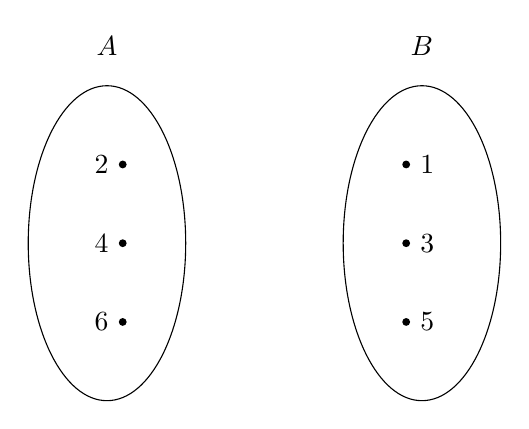
\begin{tikzpicture}[
          myPoint/.style={circle, fill, inner sep=1pt},
          myArrow/.style={->, shorten >=7.5pt, shorten <=5pt}]
          \draw (-2,0) circle [x radius=1, y radius=2];
          \node at (-2,2.5) {$A$};
          \draw (2,0) circle [x radius=1, y radius=2];
          \node at (2,2.5) {$B$};
          \node[myPoint, label={180:$2$}] (xo) at (-1.8,1) {};
          \node[myPoint, label={180:$4$}] (xt) at (-1.8,0) {};
          \node[myPoint, label={180:$6$}] (xr) at (-1.8,-1) {};
          \node[myPoint, label={0:$1$}] (fxo) at (1.8,1) {};
          \node[myPoint, label={0:$3$}] (fxt) at (1.8,0) {};
          \node[myPoint, label={0:$5$}] (fxt) at (1.8,-1) {};
%          \draw[myArrow] (xo) -- (fxt);
%          \draw[myArrow] (xt) -- (fxo);
%          \draw[myArrow] (xr) -- (fxo);
        \end{tikzpicture}
        \hspace*{15mm}
      \end{flushright}
    \task For every $(x,y)\in A\times B$, $(x,y)\in S$ means that $y=x+1$.

      \begin{flushright}
        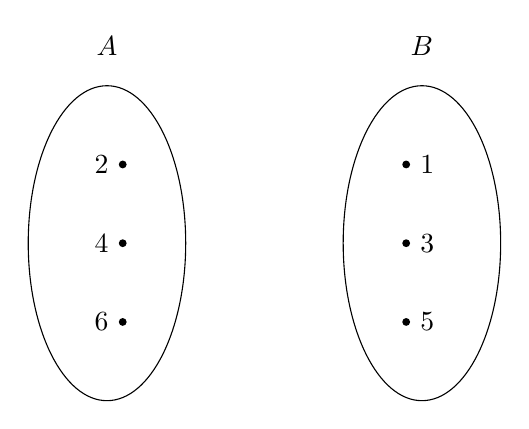
\begin{tikzpicture}[
          myPoint/.style={circle, fill, inner sep=1pt},
          myArrow/.style={->, shorten >=7.5pt, shorten <=5pt}]
          \draw (-2,0) circle [x radius=1, y radius=2];
          \node at (-2,2.5) {$A$};
          \draw (2,0) circle [x radius=1, y radius=2];
          \node at (2,2.5) {$B$};
          \node[myPoint, label={180:$2$}] (xo) at (-1.8,1) {};
          \node[myPoint, label={180:$4$}] (xt) at (-1.8,0) {};
          \node[myPoint, label={180:$6$}] (xr) at (-1.8,-1) {};
          \node[myPoint, label={0:$1$}] (fxo) at (1.8,1) {};
          \node[myPoint, label={0:$3$}] (fxt) at (1.8,0) {};
          \node[myPoint, label={0:$5$}] (fxt) at (1.8,-1) {};
%          \draw[myArrow] (xo) -- (fxt);
%          \draw[myArrow] (xt) -- (fxo);
%          \draw[myArrow] (xr) -- (fxo);
        \end{tikzpicture}
        \hspace*{15mm}
      \end{flushright}
    \task $T$ is defined by the arrow diagram
      \vspace*{-\baselineskip}

      \begin{flushright}
        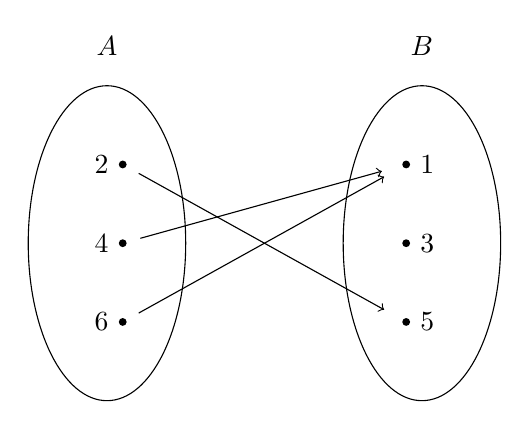
\begin{tikzpicture}[
          myPoint/.style={circle, fill, inner sep=1pt},
          myArrow/.style={->, shorten >=7.5pt, shorten <=5pt}]
          \draw (-2,0) circle [x radius=1, y radius=2];
          \node at (-2,2.5) {$A$};
          \draw (2,0) circle [x radius=1, y radius=2];
          \node at (2,2.5) {$B$};
          \node[myPoint, label={180:$2$}] (xo) at (-1.8,1) {};
          \node[myPoint, label={180:$4$}] (xt) at (-1.8,0) {};
          \node[myPoint, label={180:$6$}] (xr) at (-1.8,-1) {};
          \node[myPoint, label={0:$1$}] (fxo) at (1.8,1) {};
          \node[myPoint, label={0:$3$}] (fxt) at (1.8,0) {};
          \node[myPoint, label={0:$5$}] (fxt) at (1.8,-1) {};
          \draw[myArrow] (xo) -- (fxt);
          \draw[myArrow] (xt) -- (fxo);
          \draw[myArrow] (xr) -- (fxo);
        \end{tikzpicture}
        \hspace*{15mm}
      \end{flushright}
  \end{extasks}

  \pagebreak
\end{document}
